%% LyX 2.0.6 created this file.  For more info, see http://www.lyx.org/.
%% Do not edit unless you really know what you are doing.
\documentclass[english]{elsarticle}
\usepackage[T1]{fontenc}
\usepackage[utf8]{inputenc}
\usepackage[a4paper]{geometry}
\geometry{verbose}
\usepackage{babel}
\usepackage{amsthm}
\usepackage{amsmath}
\usepackage{amssymb}
\usepackage{graphicx}
\usepackage{esint}
\usepackage[unicode=true]
 {hyperref}

\makeatletter
%%%%%%%%%%%%%%%%%%%%%%%%%%%%%% Textclass specific LaTeX commands.
\theoremstyle{plain}
\newtheorem{thm}{\protect\theoremname}
  \theoremstyle{definition}
  \newtheorem{defn}[thm]{\protect\definitionname}
  \theoremstyle{plain}
  \newtheorem{prop}[thm]{\protect\propositionname}

%%%%%%%%%%%%%%%%%%%%%%%%%%%%%% User specified LaTeX commands.


\usepackage{babel}
\usepackage{amsthm}



\usepackage{times}%\usepackage{subfloat}
%\usepackage{subfig}
\usepackage{psfrag}\usepackage{babel}
\usepackage{times}

\def\d{\mathrm{d}}
\def\dmu{\mathrm{d}\mu}
\def\Esp{\mathbb{E}}
\def\Rset{\mathbb{R}}
\def\X{\mathcal{X}}

\newtheorem{definition}{Definition}
\newtheorem{proposition}{Proposition}

%%%

\def\ps@pprintTitle{%
  \let\@oddhead\@empty
  \let\@evenhead\@empty
  \def\@oddfoot{\reset@font\hfil\thepage\hfil}
  \let\@evenfoot\@oddfoot
}

\makeatother

  \providecommand{\definitionname}{Definition}
  \providecommand{\propositionname}{Proposition}
\providecommand{\theoremname}{Theorem}

\begin{document}

\title{T'aurais pas une entropie?}


\author{by jfb \& co \date{} }
\begin{abstract}
Where we show that it is possible to derive new entropies yielding
a particular specified maximum entropy distribution. There are (probably)
many errors --I hope not fundamental but is is possible; (certainly
many) approximations, typos, maths and language mistakes.Suggestions
and improvements will be much appreciated. 
\end{abstract}

\author{% -------------------- MaxEnt -------------------- %
}

\maketitle
\global\long\def\dmu#1{\mathrm{d}\mu(#1)}


\global\long\def\Esp#1{\mathbb{E}\left[#1\right]}


\global\long\def\E#1{\mathbb{E}\left[#1\right]}


\global\long\def\X{\mathcal{X}}



\section{Maximum entropy distributions}

Let ${\displaystyle S[f]=-\int f(x)\log f(x)\dmu x)}$ be the Shannon
entropy. Subject to $n$ moment constraints such as $\Esp{[T_{i}(x}=t_{i},\, i=1,\ldots,n$
and to normalization, it is well known that the maximum entropy distribution
lies within the exponential family 
\[
f_{X}(x)=\exp\left(\sum_{i=1}^{n}\lambda_{i}T_{i}(x)+\lambda_{0}\right).
\]
In order to recover known probability distributions (that must belong
to the exponential family), it is then sufficient to specify a set
of functions $T_{i}$, i.e., a function $T:\Rset\mapsto\Rset^{n}$
where $n$ is the number of moment constraints. This has been used
by many authors. For instance, the gamma distribution can be viewed
as a maximum entropy distribution if one knows the moments $\Esp{[X}$
and $\Esp{\log(X)}.$ In order to find maximum entropy distributions
with simpler constraints or distributions outside of the exponential
family, it is possible to consider other entropies. This is discussed
below.


\author{% -------------------- Max (h,phi)-Ent -------------------- %
}


\section{Maximum $(h,\phi)$-entropy distributions}


\author{% ---------- Definition & MaxEnt solutions
}


\subsection{Definition and maximum $(h,\phi)$-entropy solution}


\author{%\global\long\def\dmu#1{\mathrm{d}\mu(#1)}
}
\begin{defn}
Let $\phi:\Omega\subset\Rset_{+}\mapsto\Rset$ be a stricly convex
differentiable function defined on a closed convex set $\Omega$.
Then, if $f$ is a probability distribution defined with respect to
a general measure $\mu(x)$ on a set $\X$, 
\begin{equation}
H_{\phi}[f]=-\int_{\X}\phi(f(x))\dmu (x)\label{eq:phi-entropy}
\end{equation}
is the $\phi$-entropy of $f$. \label{def:phi_entropy} 
\end{defn}
Since $\phi(x)$ is convex, then the entropy functional $H_{\phi}[f]$
is concave. Also note that the composition of a concave function with
a nondecreasing concave function preserves concavity, and that composition
of a convex function with a nonincreasing convex function yields a
concave functional.

\begin{definition}%\cite{Sal93,Men97}
With the same assumption in definition~\ref{def:phi_entropy}, 
\begin{equation}
H_{h,\phi}[f]=h\left(-\int_{\X}\phi(f(x))\dmu (x)\right)\label{eq:h-phi-entropy}
\end{equation}
is called $(h,\phi)$-entropy of $f$, where 
\begin{itemize}
\item either $\phi$ is convex and $h$ concave nondecreasing 
\item or $\phi$ is concave and $h$ convex nonincreasing 
\end{itemize}
\end{definition} These $(h,\phi)$-entropies have been studied in~\citet{Sal93,MenMor97}
for instance. In these works neither concavity (resp.\ convexity)
of $h$, nor the differentiability of $\phi$ are imposed.

A useful related quantity to these entropies is the Bregman divergence
associated with $\phi$: \begin{definition} With the same assumption
in definition~\ref{def:phi_entropy}, the Bregman divergence associated
with $\phi$ defined on a closed convex set $\Omega,$ is given by
\begin{equation}
D_{\phi}(x_{1},x_{2})=\phi(x_{1})-\phi(x_{2})-\phi'(x_{2})\left(x_{1}-x_{2}\right).
\end{equation}
\label{def:Bregman} \end{definition} A direct consequence of the
strict convexity of $\phi$ is the nonnegativity of the Bregman divergence:
$D_{\phi}(x_{1},x_{2})\ge0$ with equality if and only if $x_{1}=x_{2}$.

\
 Consider the problem of maximizing entropy \eqref{eq:h-phi-entropy}
subject to constraints on some moments $\Esp{\left[T(X)\right]}$
where the normalization constraint is now included in $T$ (namely
$T_{0}(x)=1$ and $t_{0}=1$). Since $h$ is monotone, it is enough
to look for the maximum of the $\phi$-entropy \eqref{eq:phi-entropy},
\begin{equation}
\begin{cases}
\max_{f} & {\displaystyle -\int\phi(f(x))\dmu (x)}\\[2mm]
\text{s.t. } & \Esp{\left[T(X)\right]}=t
\end{cases}\label{eq:MaxEnt}
\end{equation}

\begin{prop}
\label{prop:The-probability-distribution}The probability distribution
$f_{X}$ solution of the Maximum entropy problem~\eqref{eq:MaxEnt}
satisfies the equation 
\begin{equation}
\phi'\big(f_{X}(x;t)\big)=\lambda^{t}\, T(x).\label{eq:sol-h-phi}
\end{equation}
where vector $\lambda$ is such that $\Esp{T(X)}=t$. \end{prop}
\begin{proof}
The maximization problem being concave, the solution exists and is
unique. Equation~\ref{eq:sol-h-phi} results directly from the classical
Lagrange multipliers technique. 

An alternative derivation of the result consists in checking that
the distribution (\ref{eq:sol-h-phi}) is effectively a maximum entropy
distribution, by showing that $H_{\phi}[f]>H_{\phi}[g]$ for all probability
distributions with a given (fixed) moment $\Esp{\left[T(X)\right]}.$
To this end, consider the functional Bregman divergence acting on
functions defined on a common domain $\X$: 
\[
D_{\phi}(f_{1},f_{2})=\int_{\X}\phi(f_{1}(x))\dmu (x)-\int_{\X}\phi(f_{2}(x))\dmu (x)-\int_{\X}\phi'(f_{2}(x))\left(f_{1}(x)-f_{2}(x)\right)\dmu (x).
\]
From the nonnegativity of the Bregman divergence this functional divergence
is nonnegative as well, and zero if and only if $f_{1}=f_{2}$ almost
everywhere. Define by 
\[
C_{t}=\left\{ f:\X\mapsto\Rset_{+}:\:\:\Esp{\left[T(X)\right]}=t\right\} 
\]
the set of all probability distributions defined on $\X$ with given
moments $t$. Consider now $f_{X}\in C_{t}$ such that $\phi'(f_{X}(x))=\lambda^{t}\, T(x)$
and any given function $f\in C_{t}$. Then % 
\begin{eqnarray*}
D_{\phi}(f,f_{X}) & = & \int_{\X}\phi(f(x))\dmu (x)-\int_{\X}\phi(f_{X}(x))\dmu (x)-\int_{\X}\phi'(f_{X}(x))\left(f(x)-f_{X}(x)\right)\dmu (x)\\[2mm]
 & = & -H_{\phi}[f]+H_{\phi}[f_{X}]-\int_{\X}\lambda^{t}\, T(x)\left(f(x)-f_{X}(x)\right)\dmu (x)\\[2mm]
 & = & H_{\phi}[f_{X}]-H_{\phi}[f]
\end{eqnarray*}
where we used the fact that $f$ and $f_{X}$ have the same moments
$\Esp{T(X)}=t$. By nonegativity of the Bregman functional divergence,
we finally get that 
\[
H_{\phi}[f_{X}]\ge H_{\phi}[f]
\]
for all pdf $f$ with the same moments $t$ than $f_{X}$, with equality
if and only if $f=f_{X}.$ In other words, this shows that $f_{X}$,
solution of (\ref{eq:sol-h-phi}), realizes the minimum of $H_{\phi}[f]$
over $C_{t}$. 
\end{proof}

\author{% ---------- New entropy functionals
}


\subsection{Defining new entropy functionals\label{sub:Defining-new-entropy}}

Given an entropy functional, we thus obtain a maximum entropy distribution.
There exists numerous $(h,\phi)$-entropies in the literature. However
a few of them lead to explicit forms for the maximum entropy distribution.
Therefore, it is of high interest to look for the entropies that lead
to a specified distribution as a maximum entropy solution.

Since we will look for the function $\phi$ for a given probability
distribution $f_{X}(x)$ we also see that the corresponding $\lambda$
parameters can be included in the definition of the function.

Let us recall some implicit properties of $\phi(x).$ 
\begin{itemize}
\item $\phi'(x)$ is defined on a domain included on $f_{X}(\X)$; 
\item From the strict convexity property of $\phi$, necessarily $\phi'$
is increasing. 
\end{itemize}
The identification of a function $\phi(x)$ such that a given $f_{X}(x)$
is the associated maximum entropy distribution amounts to solve (\ref{eq:sol-h-phi}),
that is 
\begin{enumerate}
\item choose $T(x)$, 
\item find $\phi'(y)$ such that 
\begin{equation}
\lambda^{t}T(x)+\mu=\phi'\left(f_{X}(x)\right)=\phi'(y)\label{eq:inv}
\end{equation}

\item integrate the result to get ${\displaystyle \phi(y)=\int\phi'(y)\d y+c}$,
where $c$ is an integration constant. The entropy being defined by
${\displaystyle H_{\phi}[f]=-\int_{\X}\phi(f(x))\dmu (x)}$, the constant
$c$ will usually be zero. % 

\item Parameters $\lambda$ may be choosen case by case in order to simplify
the expression of $\phi.$ 
\end{enumerate}
Remind that $\phi'$ must be increasing, thus, necessarily, $\lambda^{t}\, T(x)$
and $f_{X}(x)$ must have the same sense of variation. 

Observe that since we want $\phi(x)$ to be convex, which means $\phi''(x)\geq0$
for a twice differeentiable function, it is thus necessary that $\phi'(x)$
is non decreasing on $[0,$max$(f)]$. By the relation 
\begin{equation}
\phi'^{-1}\left(\lambda T(x)+\mu\right)=f_{X}(x).\label{eq:aresoudre}
\end{equation}
we have that 
\[
f_{X}'(x)=\lambda T'(x)\frac{1}{\phi''\left(\phi'^{-1}\left(\lambda T(x)+\mu\right)\right)}=\lambda T'(x)\frac{1}{\phi''\left(f_{X}(x)\right)}.
\]
Hence we get that 
\[
\phi''\left(f_{X}(x)\right)=\frac{f_{X}'(x)}{\lambda T'(x)}
\]
and we see that $f_{x}(x)$ and $T(x)$ must have the same or an opposite
variation, depending on the sign of $\lambda$. 

Examples: if $\lambda$ is negative, then 
\begin{itemize}
\item for $T(x)=x,$ $f_{X}(x)$ must be non increasing,
\item for $T(x)=x^{2}$ or $T(x)=|x|,$ $f_{X}(x)$ must be unimodal with
a maximum at zero. 
\end{itemize}
For instance, for one moment constraint, if $\lambda_{1}$ is negative,
then 
\begin{itemize}
\item for $T_{1}(x)=x,$ $f_{X}(x)$ must be decreasing, %non increasing,

\item for $T_{1}(x)=x^{2}$ or $T_{1}(x)=|x|,$ $f_{X}(x)$ must be unimodal
with a maximum at zero. 
\end{itemize}
Equation~\eqref{eq:sol-h-phi} may have no solution, when $\lambda^{t}\, T(x)$
has not the same variations than $f_{X}$. But it can also have several
solutions.


\author{% -------------------- Fisher -------------------- %
}


\section{$\phi$-escort, $\phi$-Fisher information and generalized Cramér-Rao
inequality}


\author{% -------------------- Examples -------------------- %
}


\section{Some examples}


\author{% ---------- Normal
}


\subsection{Normal distribution and second-order moment}


\author{% ---------- q-exponential
}


\subsection{$q$-exponential distribution and first-order moment}


\author{% ---------- q-Normal
}


\subsection{$q$-Normal distribution and second-order moment}


\author{% ---------- q-Normal
}


\subsection{Hyperbolic secant distribution and first-order moment}

Let us consider some specific cases. 
\begin{enumerate}
\item For a normal distribution, $f_{X}(x)=\frac{1}{\sqrt{2\pi}}\exp(-\frac{x^{2}}{2})$
and $T(x)=x^{2},$ we begin by computing the inverse $y=\frac{1}{\sqrt{2\pi}}\exp(-\frac{x^{2}}{2})$,
which gives $-\frac{1}{2}x^{2}-\log\sqrt{2\pi}=\log(y).$ Choosing
$\lambda=-\frac{1}{2}$, $\mu=-\log\sqrt{2\pi}$ and integrating,
we obtain 
\[
\phi(y)=y\log y-y
\]

\item For a Tsallis $q$-exponential, $f_{X}(x)=C_{q}\left(1-(q-1)\beta x\right)_{+}^{\frac{1}{(q-1)}},$
$x\geq0,$ and $T(x)=x$. We simply have $C_{q}^{q-1}\left(1-(q-1)\beta x\right)=y^{q-1}$.
With $\lambda=qC_{q}^{q-1}\beta$ and $\mu=qC_{q}^{q-1}/(1-q)$, this
yields 
\[
\phi(y)=\frac{y^{q}}{1-q}.
\]
Taking $\mu=\left(qC_{q}^{q-1}+1\right)/(1-q)$ gives 
\[
\phi(y)=\frac{y^{q}-y}{1-q},
\]
and an associated entropy can be 
\[
H_{\phi}[f]=\frac{1}{1-q}\left(\int f(x)^{q}\text{d}\mu(x)-1\right),
\]
which is nothing but Tsallis entropy.%
\footnote{Of course, we can also take the first $\phi(y)=\frac{y^{q}}{1-q},$
integrate and add any constant, since adding a constant do not modify
the actual value af the minimizer (or maximizer if we consider concave
entropies). %
} 
\item The same entropy functional can readily be obtained for the so-called
$q$-Gaussian, or Student-t and -r distributions $f_{X}(x)=C_{q}\left(1-(q-1)\beta x^{2}\right)_{+}^{\frac{1}{(q-1)}}.$
It suffices to follow the very same steps as above with $T(x)=x^{2}.$ 
\item Let $f_{X}(x)$ be the hyperbolic secant distribution, with density
\[
f_{X}(x)=\frac{1}{2}\text{sech}(\frac{\pi}{2}x)=\frac{1}{2}\cosh^{-1}(\frac{\pi}{2}x).
\]
Obviously, $\frac{\pi}{2}x=\cosh(2y)=\phi'(y)$ with $T(x)=x$, $\lambda=\frac{\pi}{2}$,
and 
\[
\phi(y)=\sinh(2y).
\]
So doing, we obtain an hyperbolic sine entropy with the hyperbolic
secant distribution as the associated maximum entropy distribution. 
\end{enumerate}

\section{Multiform entropies}

Of course, the preceeding derivations require that (\ref{eq:inv})
is effectively solvable. In addition, one has also to choose or design
a specific $T(x)$ statistic, as well as the parameters $\lambda$
and $\mu$. In the examples above, we used $T(x)=x$ and $T(x)=x^{2}.$
Particular choices such as $T(x)=x^{2}$ or $T(x)=|x|$ obviously
lead to symmetrical densities. 

For nonsymmetrical unimodal densities, the situation is more involved.
For instance, if we take $T(x)=x$, then the resolution of (\ref{eq:inv})
amounts to compute the inverse relation of $y=f_{X}(x)$, which is
is multi-valued. Indeed, $f_{X}(x)$ is not injective and to each
$y$ correspond two distinct values of $x.$ Let us denote $\mathcal{S}_{y}$
the image of $f_{X}$, $I_{+}\subseteq\mathbb{R}$ the domain where
$f_{X}(x)$ is non decreasing, and $I_{-}\subseteq\mathbb{R}$ the
domain where $f_{X}(x)$ is non increasing. We thus have two possible
inverses defined respectively say $\phi_{+}':\mathcal{S}_{y}\mapsto I_{+}$
and $\phi_{-}':\mathcal{S}_{y}\mapsto I_{-}$ such that $\phi_{+}'^{-1}(-x)=f_{X}(x)$
for $x\in I_{+}$ and $\phi_{-}'^{-1}(-x)=f_{X}(x)$ for $x\in I_{-}$.
Furthermore, by the remarks at the end of section \ref{sub:Defining-new-entropy},
we see that $\phi_{+}$ is convex while $\phi_{-}$is concave. In
this context, our proposal is to define a $\phi$-entropy as follows
\[
H_{\phi}[f_{X}]=-\int_{I_{+}}\phi_{+}\left(f_{X}(x)\right)\dmu x-\int_{I_{-}}\phi_{-}\left(f_{X}(x)\right)\dmu x.
\]
It is easy to check that this entropy functional is no more convex
nor concave (for the subset of distributions with support on $I_{+}$the
entropy is convex while it its concave for on the subset of distributions
on $I_{-}$. We propose to look for the \emph{extreme entropy} (instead
of the maximum entropy as in the classical case). With a moment constraint,
the Lagrangian is 
\[
L\left(f_{X};\lambda_{1},\lambda_{0}\right)=\int_{I_{+}}\phi_{+}\left(f_{X}(x)\right)\dmu x+\int_{I_{-}}\phi_{+}\left(f_{X}(x)\right)\dmu x+\int_{\mathbb{R}}\lambda_{1}x\,\dmu x+\int_{\mathbb{R}}\lambda_{0}\,\dmu x
\]
and its first variation is
\[
\delta L\left(f_{X};\lambda_{1},\lambda_{0}\right)=\phi_{+}\left(f_{X}(x)\right)1_{I_{+}}+\phi_{-}\left(f_{X}(x)\right)1_{I_{-}}+\lambda_{1}x+\lambda_{0}.
\]
Thus the critical points are defined by $\phi_{+}\left(f_{X}(x)\right)+\lambda_{1}x+\lambda_{0}=0$
for $x\in I_{+}$and $\phi_{-}\left(f_{X}(x)\right)+\lambda_{1}x+\lambda_{0}=0$
for $x\in I_{-}$, which actually define the extreme entropy distribution
$f_{X}(x)$ as the inverse relation of a multiform entropy. Obviously,
this formulation includes the classical maximum entropy approach as
a particular case. 

Observe that it is still possible to get a maximum or a minimum entropy
solution, but on subsets. Thus, it will still be possible to use these
entropies in testing problems. For such goal, define $m_{+}$ to be
the moment computed on the subset $I_{+}:$ $m_{+}=\int_{I_{+}}x\, f_{X}(x)\dmu x,$
and similarly for a moment $m_{-}$ computed on $I_{-}$. By the very
same reasoning and proof as in the classical case (see the proof of
proposition \ref{prop:The-probability-distribution}), we have that 
\begin{itemize}
\item (a) $H_{\phi_{+}}[f_{X}]\ge H_{\phi_{-}}[f_{1}]$ for all distributions
$f_{1}$ with a fixed moment $m_{+},$
\item (a) $H_{\phi_{-}}[f_{X}]\leq H_{\phi_{-}}[f_{2}]$ for all distributions
$f_{2}$ with a fixed moment $m_{-}$
\end{itemize}
where $f_{X}(x)=\phi_{+}'^{-1}(-x)$ for $x\in I_{+}$ and $f_{X}(x)=\phi_{-}'^{-1}(-x)$
for $x\in I_{-}$. Hence we will be able to use these entropies for
distribution testing, provided that we are able to compute empirical
values for $m_{+}$ and $m_{-}$ from data, which is quite easy. 


\subsection{Example 1. The logistic distribution}

The pdf of the logistic distribution is given by 
\[
f_{X}(x)=\frac{e^{-\frac{x}{s}}}{s\left(1+e^{-\frac{x}{s}}\right)^{2}}.
\]
This distribution, which resembles the normal distribution but has
heavier tails, has been used in many applications. By direct calculations,
we obtain 
\[
\begin{cases}
\phi_{-}'(y)= & s\ln\left(\frac{1}{2}\,{\frac{-2\, ys+1+\sqrt{-4\, ys+1}}{ys}}\right),\\
\phi_{+}'(y)= & s\ln\left(-\frac{1}{2}\,{\frac{2\, ys-1+\sqrt{-4\, ys+1}}{ys}}\right).
\end{cases}
\]


The associated entropy is then 

\[
\begin{cases}
 & \phi_{-}(y)=-\frac{1}{2}\,\sqrt{-4\, ys+1}+\frac{1}{2}+ys\,\ln\left(-{\frac{\sqrt{-4\, ys+1}-1}{\sqrt{-4\, ys+1}+1}}\right)\\
 & \phi_{+}(y)=\frac{1}{2}\,\sqrt{-4\, ys+1}+\frac{1}{2}+ys\,\ln\left(-{\frac{\sqrt{-4\, ys+1}-1}{\sqrt{-4\, ys+1}+1}}\right)
\end{cases}
\]
for $y\in[0,\frac{1}{4s}],$ and where we have introduced a integration
constant such that $\min_{y}\phi_{+}(y)=0.$ For $y>\frac{1}{4s},$
we extend the function and let $\phi_{+}(y)=+\infty.$ Figure \ref{fig:Entropy-logistic}
\begin{figure}
%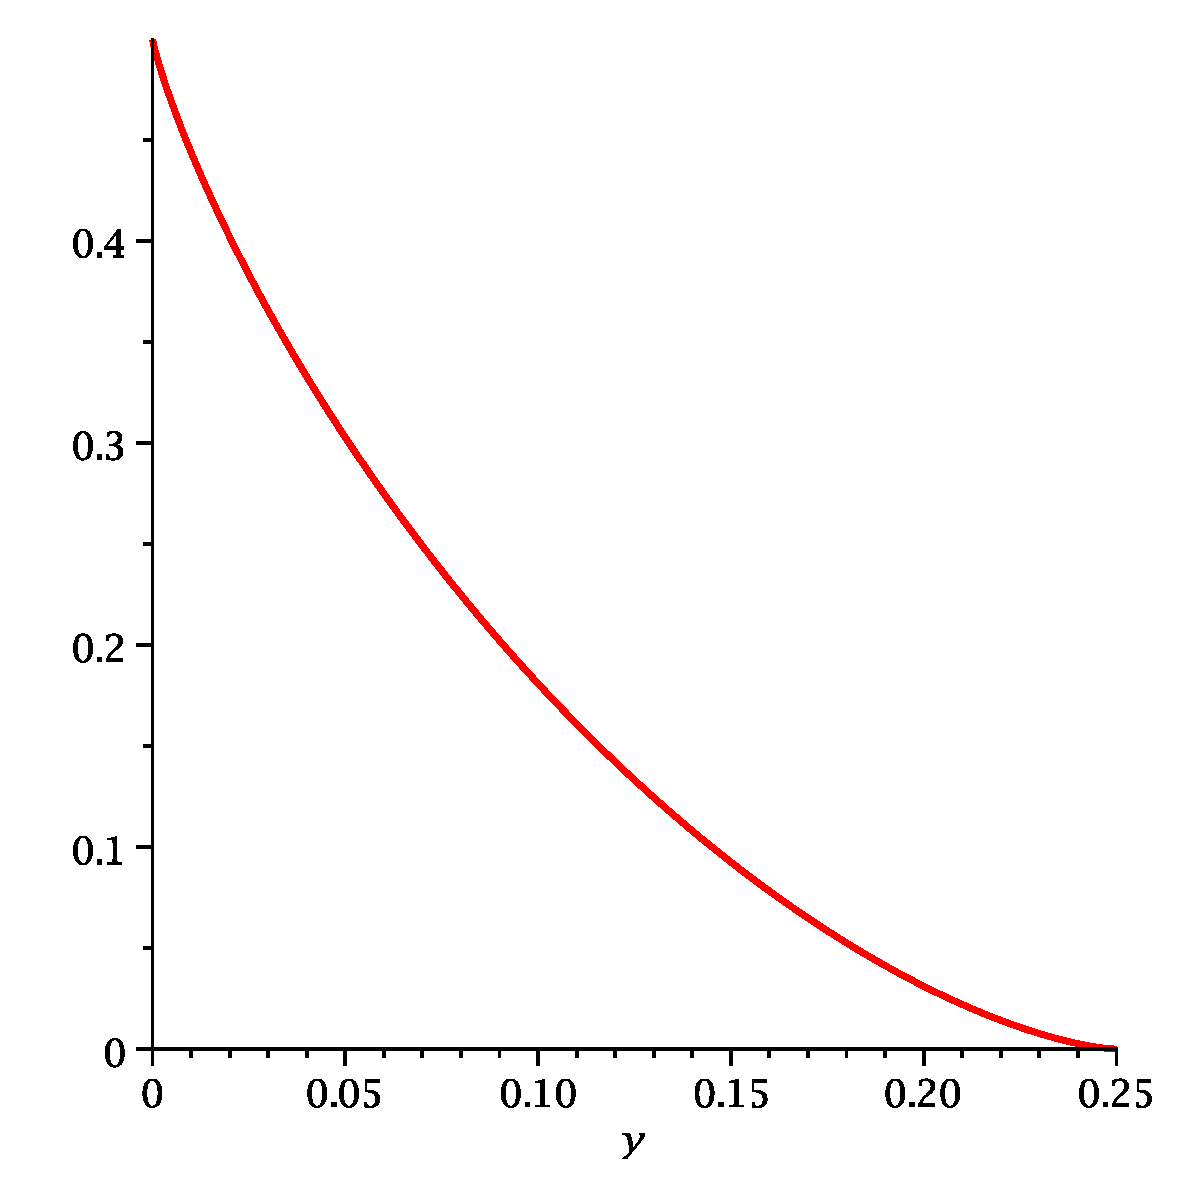
\includegraphics[width=5cm]{maple/phi_logistic}\caption{Entropy derived from the logistic distribution. \label{fig:Entropy-logistic}}
\end{figure}
 gives a representation of this entropy for $s=1.$


\subsection{Example 2. The gamma distribution}

The probability density function of the gamma distribution is given
by 
\[
f_{X}(x)=\frac{{\beta}^{\alpha}{x}^{\alpha-1}{e}^{-\beta\, x}}{\Gamma\left(\alpha\right)}
\]


We obtain 
\[
\phi'(y)=-{{\rm e}^{\frac{1}{\alpha-1}\left(-{\it W}\left(-{\frac{\beta\,\left(y\Gamma\left(\alpha\right){\beta}^{-\alpha}\right)^{\left(\alpha-1\right)^{-1}}}{\alpha-1}}\right)\alpha+{\it W}\left(-{\frac{\beta\,\left(y\Gamma\left(\alpha\right){\beta}^{-\alpha}\right)^{\left(\alpha-1\right)^{-1}}}{\alpha-1}}\right)+\ln\left(y\Gamma\left(\alpha\right){\beta}^{-\alpha}\right)\right)}},
\]
where ${\it W}$ is the Lambert W multivalued `function' defined by
$z=W(z)e^{W(z)}$ (ie the inverse relation of $f(w)=we^{w}$). Unfortunately,
in the general case, we do not have a closed form for $\phi(y)$ as
the integral of $\phi'(y)$.%
\footnote{This might not be completely unacceptable. Indeed, it is really not
difficult to compute numerically the values of $\phi(y).$%
} Restricting us to the case $\alpha=2$, we have 
\[
\phi(y)=\frac{\left(1-{\it W}\left(-{\frac{y}{\beta}}\right)+y\left({\it W}\left(-{\frac{y}{\beta}}\right)\right)^{2}\right)}{{\it \beta\, W}\left(-{\frac{y}{\beta}}\right)}+\frac{\beta}{e},
\]
which is convex if we choose the -1 branch of the Lambert function
and concave for the 0 branch. An example with $\alpha=2$ and $\beta=3$
is given on Figure \ref{fig:Entropy-gamma}. 
\begin{figure}
%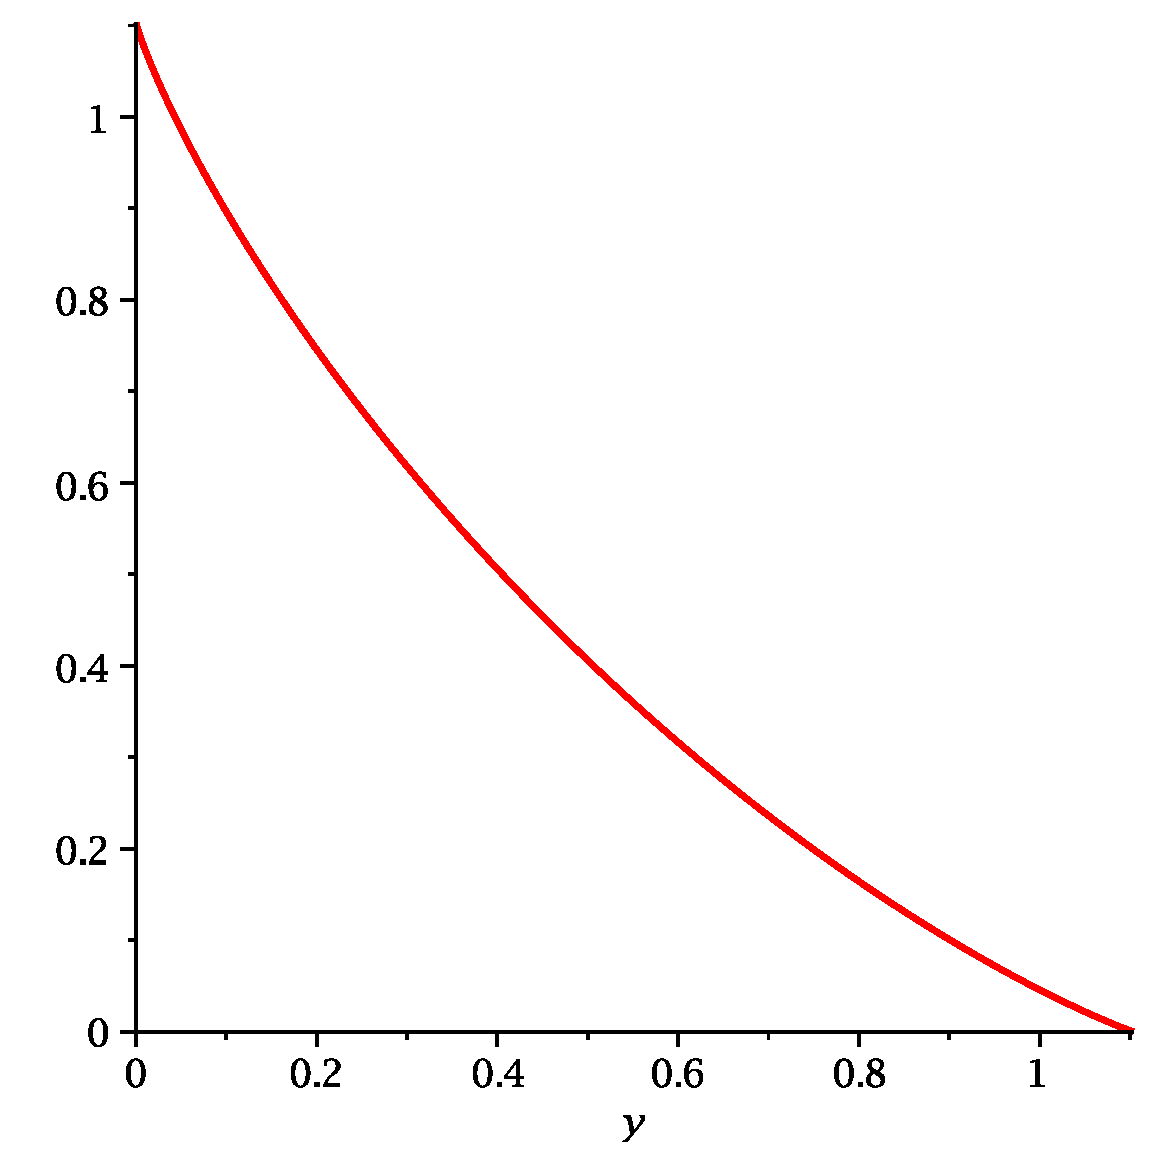
\includegraphics[width=5cm]{maple/phi_gamma}\caption{\label{fig:Entropy-gamma}Entropy derived from the gamma distribution}
\end{figure}



\subsection{Example 3. The arcsine distribution}

As a further example, we consider the case of the arcsine distribution
(see \href{http://en.wikipedia.org/wiki/Arcsine_distribution}{wiki})
which also yields a multiform entropy. This distribution, defined
for $x\in(0,1),$ is a special case of the Beta distribution with
parameters $\alpha=\beta=1/2.$ It has the following pdf: 
\[
f_{X}(x)=\frac{1}{\pi\sqrt{x(1-x)}}.
\]
Observe that $\min_{x}f_{X}(x)=2/\pi.$ Doing our now usual calculations,
we obtain 
\[
\begin{cases}
\phi_{-}'(y)= & -\frac{\, y\pi+\,\sqrt{{y}^{2}{\pi}^{2}-4}}{2y\pi},\\
\phi_{+}'(y)= & -\frac{\, y\pi-\,\sqrt{{y}^{2}{\pi}^{2}-4}}{2y\pi}.
\end{cases}
\]
and the expression of the entropy is 
\[
\phi_{\pm}(y)=\frac{1}{2}\,{\frac{\sqrt{{y}^{2}{\pi}^{2}-4}}{\pi}}\pm\frac{1}{\pi}\arctan\left(2\,{\frac{1}{\sqrt{{y}^{2}{\pi}^{2}-4}}}\right)-\frac{1}{2}\, y,
\]
for $y\geq1/\pi$. The entropy is shown on \ref{fig:arcseine entropy}.
\begin{figure}
%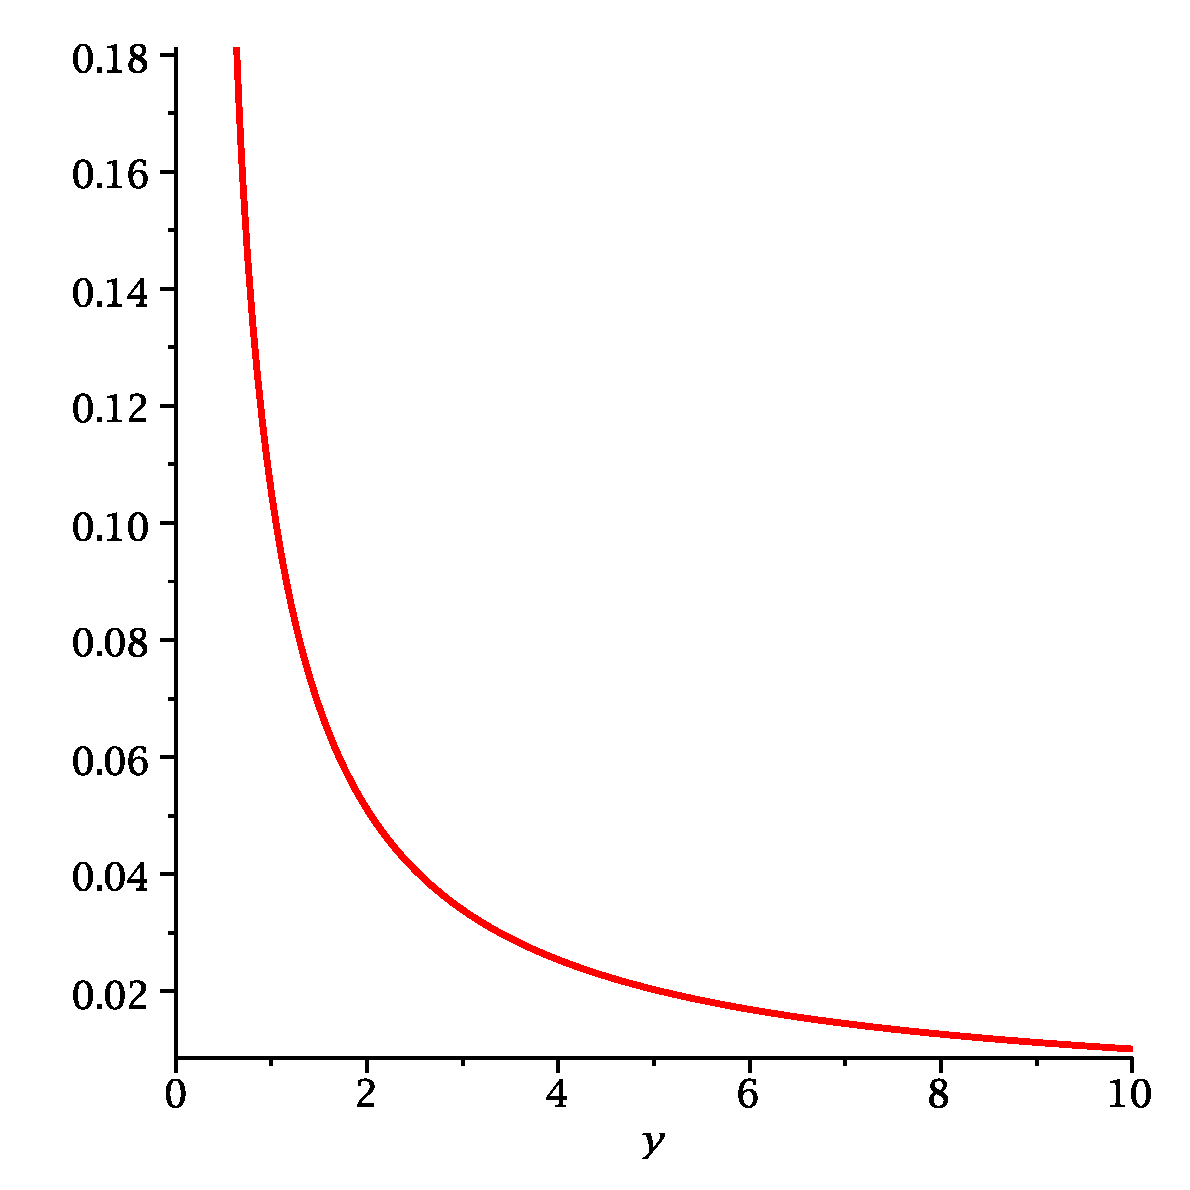
\includegraphics[width=5cm]{maple/phi_arcsine}\caption{The entropy associated with an arcsine distribution. \label{fig:arcseine entropy}}
\end{figure}



\subsection{Example 4. The Chi-squared distribution}

Let us now consider the case of a chi-squared distribution. The probability
density, for $x\geq0,$is given by
\[
f_{X}(x)=c\, x^{\frac{k}{2}-1}\exp-\frac{x}{2}
\]
with $c^{-1}=2^{\frac{k}{2}}\Gamma(\frac{k}{2})$. Instead of $T(x)=x,$
we now take $T(x)=x^{2}$ and $\lambda=1,$ which means that we look
for $\phi$ such that $\phi'^{-1}(x^{2})=f_{X}(x)$. Solving, we get
that
\[
\phi'(y)=\begin{cases}
4\left(n-1\right)^{2}W\left(\frac{1}{2(n-1)}\left(-y\right)^{\frac{1}{n-1}}\right)^{2} & \text{for \ensuremath{k}=\ensuremath{2n}even, \ensuremath{n}even}\\
4\left(n-1\right)^{2}W\left(\pm\frac{1}{2(n-1)}\left(y\right)^{\frac{1}{n-1}}\right)^{2} & \text{for \ensuremath{k}=\ensuremath{2n}even, \ensuremath{n}odd}\\
\left(k-2\right)^{2}W\left(\frac{1}{k-2}\left(-y^{2}\right)^{\frac{1}{k-2}}\right)^{2} & \text{for \ensuremath{k}odd}
\end{cases}
\]


Among these solutions, we must discard complex valued solutions. Since
$y$ is non negative, we see that we can only keep solutions with
$k=2n$ even with $n$ odd (or $n=2$). For $n=2$, the solution reduces
to
\[
\phi'(y)=4W\left(-\frac{1}{2}y\right)^{2}.\text{ }
\]


By integration, we obtain the corresponding entropy, e.g. 
\[
\phi(y)=4\,{\frac{\left(-4+4\,{\it W}\left(-1/2\, y\right)-2\,\left({\it W}\left(-1/2\, y\right)\right)^{2}+\left({\it W}\left(-1/2\, y\right)\right)^{3}\right)y}{\left(-1/2\, y\right)}}\text{ for n=2}
\]



\end{document}
